\section{Our Approach}
In this section, we present a novel approach to model and verify the properties of co-simulation with TA. Besides, we propose encoding rules to encode FMU into timed automata. In next section, we will encode the FMUs of our case study with the network of TA, so that we can verify the case study with the model checker UPPAAL.
\label{sec:encoding}
\subsection{Framework of our approach}
The schematic view of our approach is shown in Fig.~\ref{paper-arc}. At the \textbf{design phase}, we construct the architecture of CPSs with SysML Block Diagrams (BDD) \cite{RahimHI17} and SysML connector. Each block represents a component and the communication between components is modelled with SysML connector. To simulate the whole system with co-simulation techniques, the block can be modelled with a FMU and the connector can be described with connector configuration. Besides, we design MA to accomplish the communication between FMUs. It is the \textbf{simulation phase} in our framework. Before simulating the system, we need to ensure the coordination (connector configuration and MA) of system is correct. To verify the correctness of the coordination, we encode each FMU component and model the master algorithm by timed automaton, and we translate connector cofiguration to the channel between timed automata.  By this way, we can obtain the network of timed automata composed with timed automata and channel. Therefore, some properties (e.g. livelock or deadlock) of the network of timed automata can be verified using model checker UPPAAL \cite{BehrmannDLHPYH06}. Once ensuring the correctness of coordination, we can using co-simulation engine to simulate the whole system and obtain the simulation trace. In this paper, we focus on how to ensure the correctness of coordination which is the verification phase in Fig.~\ref{paper-arc}.
\begin{figure}[htbp]
	\centering	{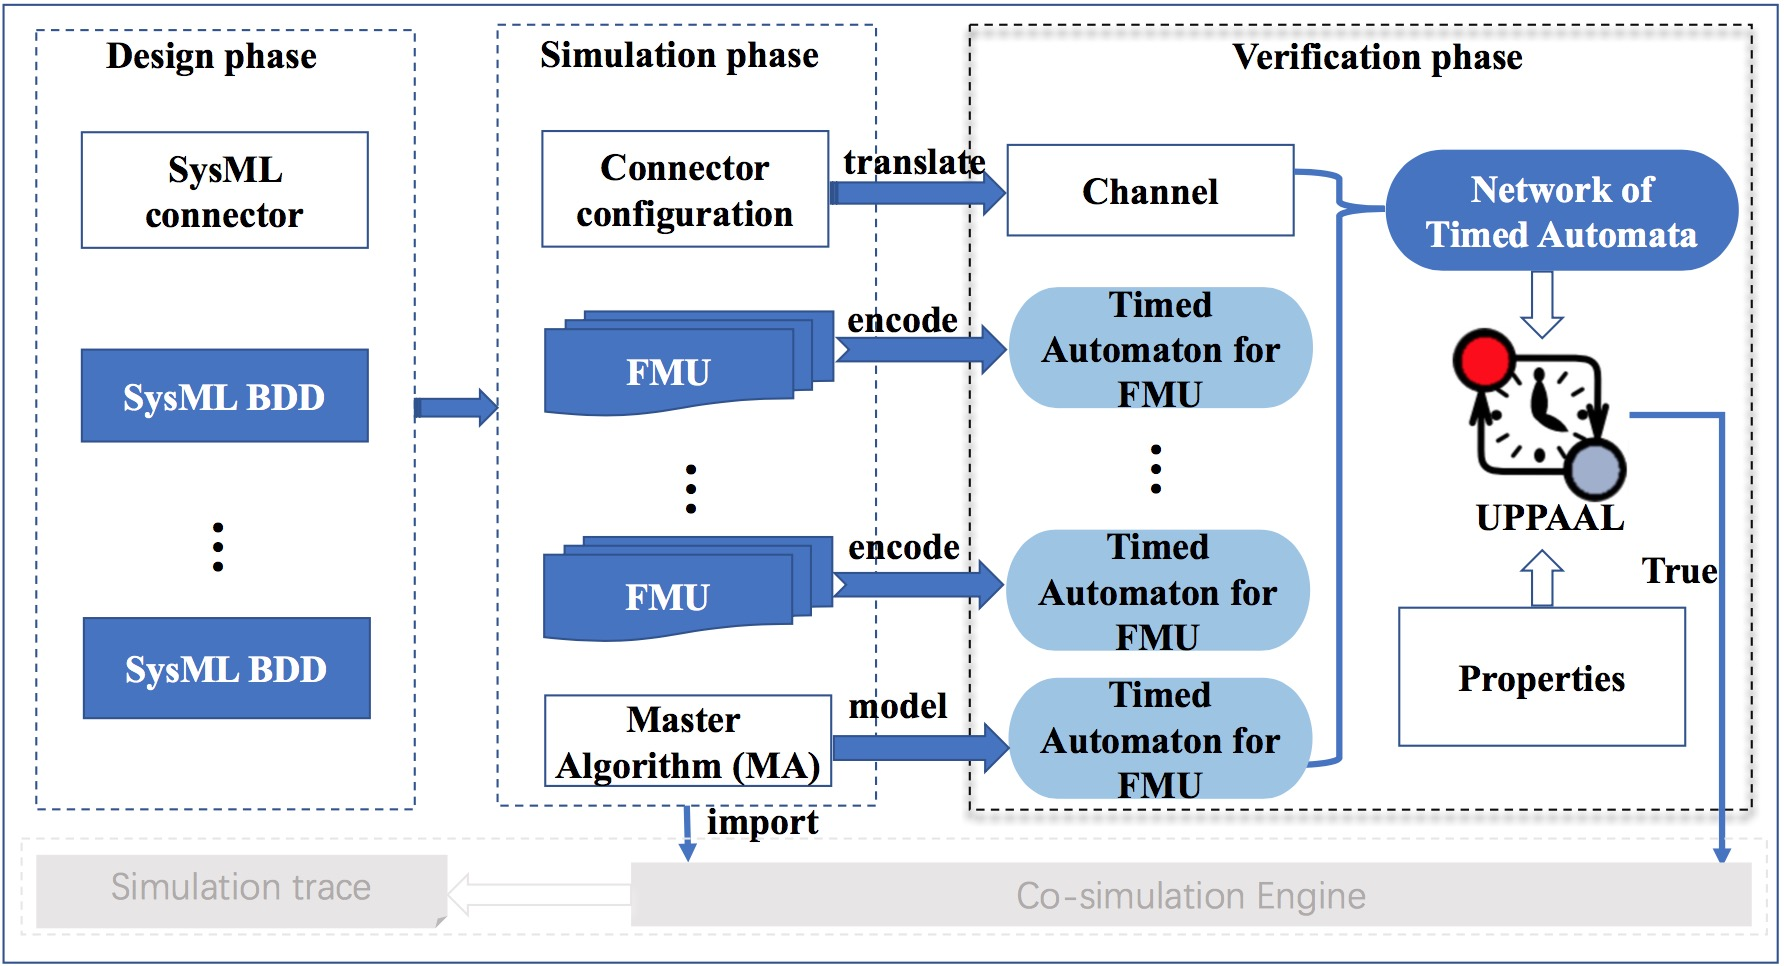
\includegraphics[width=3.5in,height=2.0in]{fig/approachnew.png}}
	\caption{A schematic view of our approach.}
	\label{paper-arc}
\end{figure}

\subsection{Encoding FMUs into timed automata}
We find that there is a semantic gap between FMU and TA. The former focus on the execution sequence of FMU, which specifies the state change process with time elapsing. Essentially, the execution trace of TA is semantic equivalence to the execution sequence of FMU. Therefore, we can encode FMU into TA to analyse the behavior of FMU components without exploring its internal structure. 
Given an FMU $F=(S,U,Y,D,s_{0},set,get,doStep)$, we encode the FMU into a timed automaton $\textit{A}=(L,l_{0},E,I)$ , the congruent relationships between them are as following:
\begin{itemize}
\item
$L$ is a set of finite locations. Note that the state of the transition system $L_{\textit{A}}$ can be seen as the state of $F$, i.e., $(l,v) \rightarrow s$.
\item
The initial state of the transition system $L_{\textit{A}}$ can be seen as the initial state of $F$, i.e., $(l_{0},v_{0}) \rightarrow s_{0}$. 
\item
Each input variable $u \in U$ ranges over $Act_{i} \cup \{absent\}$.
\item
Each output variable $y \in Y$ ranges over $Act_{o} \cup \{absent\}$.
\item
An input action $e \in Act_{i}$ is such that the function $set$ of $F$ sets the input variable $u$ with a given value. 
\item
An output action $e \in Act_{o}$ indicates that the function $get$ of $F$ gets the output variable $y$. The set of values in the $Act_{i}$ can be seen as $Y$ of $F$.  
\item
The communication between the network of TA is the same as the I/O dependencies information in FMU. $(u,y) \in D$ denotes that output $y$ depend on input $u$. The output actions also depend on the input actions in TA.
\item
For any $e \in Act$ of A, there is a transition $s \xrightarrow{e} s^{\prime}$, which may be found after the function $doStep$ is executing. For instance, if there is a transition $l \xrightarrow{e} l^{\prime}$ in $A$, at the same time $doStep(s,h)$ may be called which indicates that $F$ accepts the time step $h$ and reaches the new state $s^{\prime}$. However, $F$ maybe rejects the time step, if there is a rollback behavior happens, the transition in TA could be an edge $l^{\prime} \xrightarrow{e} l$, which denotes that a location travels to the former location.

\end{itemize}
\begin{figure}[htbp]
	\centering	{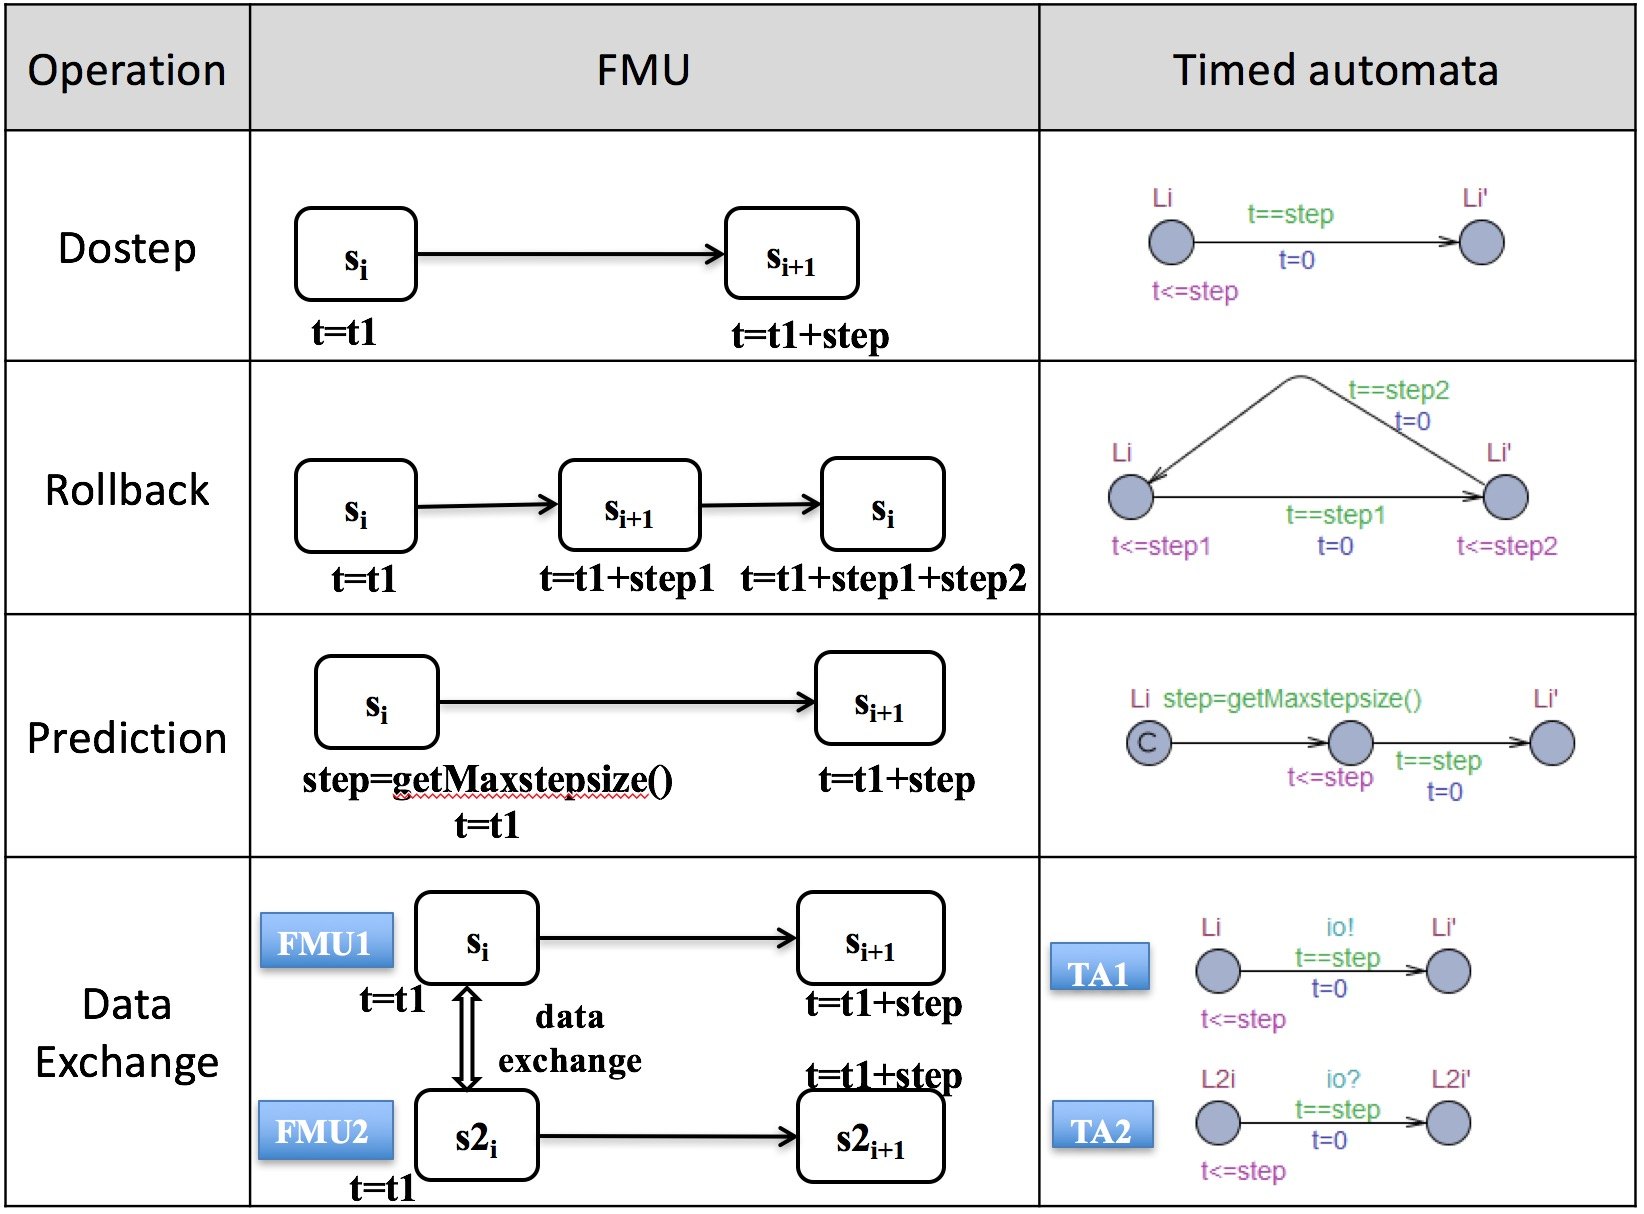
\includegraphics[width=3.5in,height=2.5in]{fig/abstractRole.png}}
	\caption{Encoding rules from FMU to TA.}
	\label{fmutota}
\end{figure}

It is not easy to translate FMU to TA directly. Inspired by \cite{Tripakis15}, we propose some encoding rules according to the congruent relationships. As we can see in the Fig.~\ref{fmutota}, given a state $s_{i}$ at $t_{1}$ in FMU, the operation $Dostep$ makes FMU reach a new state $s_{i+1}$ at $t_{1}+step$. This situation can be encoded into a transition in TA, in which a location $L_{i}$ delays $step$ time and goes to a new location $L_{i}^{\prime}$.

For the operation $Rollback$, given a state $s_{i}$ at $t_{1}$ in FMU, the FMU will do a \emph{step1} to $s_{i+1}$ at $t_{1}+step1$, and then, the operation $rollback$ makes FMU reach the former state $s_{i}$. For this situation, it can be encoded as: location $L_{i}$ delays \emph{step1} units time and reach a new location $L_{i}^{\prime}$ after a transition, and then returns to the former Location $L_{i}$. 

For the operation $prediction$, given a state $s_{i}$, FMU can get max step size \emph{step} for next step, and then reach a new state $s_{i+1}$ at $t_{1}+step$. For TA, it gets max step size in location $L_{i}$, then it delays $step$ units time and reach a new location $L_{i}^{\prime}$ .

For data exchange between two FMUs in state $s_{i}$ at $t_{1}$, they exchange data at $t_{1}$ and then do the same step to $s_{i+1}$. In TA, there will be a signal \emph{io} to make the two FMUs do the same step from $L_{i}$ to $L_{i+1}$ after data exchange.

Although there are semantic gaps between FMUs and timed automata, we provide appropriate encoding rules to formalism FMU with timed automata. It lays the foundation to analyse FMI co-simulation with timed automata-based model checking. 
%Limited to the length of this paper, we don't prove the correctness of encoding rules. But the encoding process is semantic-preserve. In section \ref{sec:sysml}, we apply these encoding rules to the water tank case study. According to the simulation results, we can find that the encoding rules work well.
As for the correctness of encoding rules, we analyse the equivalence of execution fragment. For the encoding rule of $Dostep$ operation, we can obtain the execution fragments of FMU and timed automata, which are fragments ($s_{i}$, $t_{1}$), ($s_{i+1}$, $t_{1}+step$) and ($l_{i}$, $t$), ($l_{i}^{\prime}$, $t+step$). It means that TA and FMU execute $step$ units time, and jump to a new state or location.  For encoding rule of $Rollback$ operation, we can obtain the execution fragment of FMU and timed automata, which are fragments ($s_{i}$, $t_{1}$), ($s_{i+1}$, $t_{1}+step1$), ($s_{i}$, $t_{1}+step1+step2$) and ($l_{i}$, $t$), ($l_{i}^{\prime}$, $t+step1$), ($l_{i}$, $t+step1+step2$). It means that TA and FMU execute $step1$ units time, and jump to a new state or location, and then execute $step2$ units time, return to previous state or location. For the encoding rule of $Prediction$, the execution fragments of FMU and timed automata are ($s_{i}$, $t_{1}$), ($s_{i+1}$, $t_{1}+step$) and ($l_{i}$, $t$), ($l_{i}^{\prime}$, $t+step$). For the encoding rule of $Data Exchange$ operation, the execution fragments of FMU1 and TA1 are ($s_{i}$, $t_{1}$), ($s_{i+1}$, $t_{1}+step$) and ($l_{i}$, $t$), ($l_{i}^{\prime}$, $t+step$). The execution fragments of FMU2 and TA2 are  ($s2_{i}$, $t_{1}$), ($s2_{i+1}$, $t_{1}+step$) and ($l2_{i}$, $t$), ($l2_{i}^{\prime}$, $t+step$). We have  analysed the whole execution trace of FMU and timed automata for these encoding rules. We find that the execution trace of FMU and timed automata are equivalent. By the analyzing the equivalence of execution traces, the correctness of encoding rules are proved. In section \ref{sec:sysml}, we apply these encoding rules to the water tank case study. According to the simulation results of the case study, we also find that the encoding rules work well.